\documentclass[11pt]{article}
\usepackage[margin=0.9in]{geometry}
\usepackage{xcolor}
\usepackage{graphicx}
\usepackage{tabularx}
\usepackage{booktabs}
\usepackage{parskip}
\usepackage{listings}
\usepackage[colorlinks=true,urlcolor=blue,linkcolor=black]{hyperref}
\usepackage{tikz}
\usetikzlibrary{positioning,arrows.meta}

\definecolor{bg}{gray}{0.96}
\lstset{basicstyle=\ttfamily\footnotesize,backgroundcolor=\color{bg},frame=single,
  framesep=5pt,rulecolor=\color{gray!40},breaklines=true,columns=fullflexible,
  xleftmargin=5pt,xrightmargin=5pt}
\newcommand{\yes}{\textcolor{green!55!black}{\textbf{Yes}}}
\newcommand{\done}{\textcolor{green!55!black}{\textbf{Done}}}

\title{\vspace{-1.5em}ALBATROSS --- System Architecture \& Review Response\\
\large PX4 SITL + Gazebo (Chattogram) + ROS 2 autonomy + web GCS}
\author{}
\date{\today}

\begin{document}
\maketitle
\vspace{-2em}

\section{System Architecture}
A full software-in-the-loop autonomous maritime-patrol simulator. The autonomy
stack builds exclusion-aware waypoints, the flight controller flies them, Gazebo
renders the vehicle over the real Chattogram port terrain, and a browser-based
Ground Control Station (GCS) provides live ops: map, 3D view, chase-camera feed,
and a multi-waypoint mission editor.

\begin{center}
\resizebox{\textwidth}{!}{%
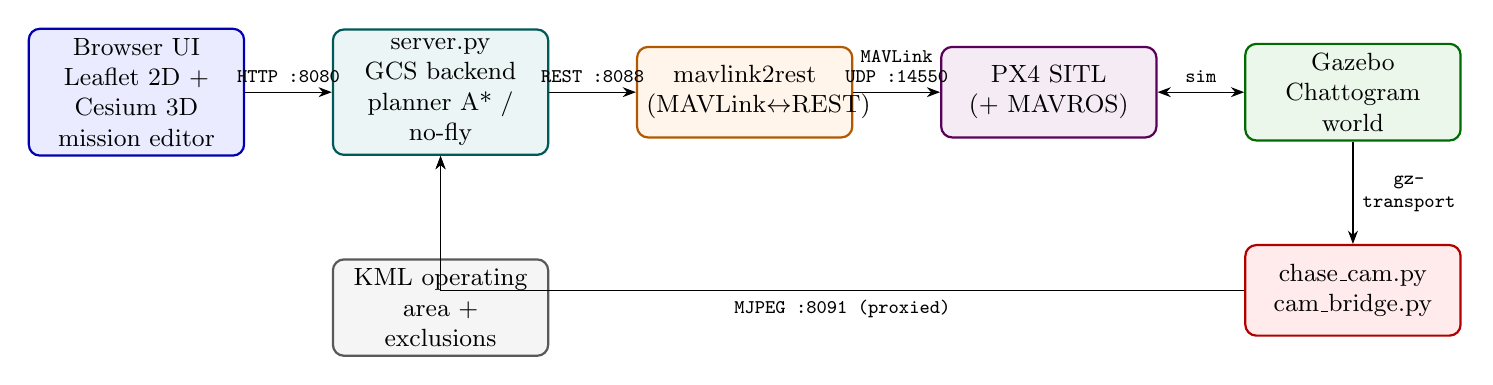
\begin{tikzpicture}[>=Stealth, node distance=1.0cm and 1.1cm,
  box/.style={rectangle, rounded corners, draw=#1!70!black, fill=#1!8, thick,
    align=center, text width=2.5cm, minimum height=1.15cm, font=\small},
  lab/.style={font=\scriptsize\ttfamily, midway, above}]
  \node[box=blue]  (ui)  {Browser UI\\Leaflet 2D +\\Cesium 3D\\mission editor};
  \node[box=teal, right=of ui]  (gcs) {server.py\\GCS backend\\planner A* /\\no-fly};
  \node[box=orange, right=of gcs](m2r) {mavlink2rest\\(MAVLink$\leftrightarrow$REST)};
  \node[box=violet, right=of m2r](px4) {PX4 SITL\\(+ MAVROS)};
  \node[box=green!60!black, right=of px4](gz) {Gazebo\\Chattogram\\world};
  \node[box=red, below=1.3cm of gz] (cam) {chase\_cam.py\\cam\_bridge.py};
  \node[box=gray, below=1.3cm of gcs] (kml) {KML operating\\area +\\exclusions};

  \draw[->] (ui)  -- node[lab]{HTTP :8080} (gcs);
  \draw[->] (gcs) -- node[lab]{REST :8088} (m2r);
  \draw[->] (m2r) -- node[lab]{\shortstack{MAVLink\\UDP :14550}} (px4);
  \draw[<->](px4) -- node[lab]{sim} (gz);
  \draw[->] (gz)  -- node[lab, right]{\shortstack{gz-\\transport}} (cam);
  \draw[->] (kml) -- (gcs);
  \draw[->] (cam) -| node[lab, near start, below]{MJPEG :8091 (proxied)} (gcs);
\end{tikzpicture}}
\end{center}

\subsection{Components}
\begin{itemize}\setlength\itemsep{1pt}
  \item \textbf{PX4 SITL + Gazebo} --- flight dynamics + rendering of the x500 over
        the real Chattogram satellite/terrain world (\texttt{PX4\_GZ\_WORLD=chattogram}).
  \item \textbf{maritime\_autonomy} (ROS 2 pkg) --- \texttt{planner.py} (A* over the KML
        operating area, exclusion-aware, no-fly enforced), \texttt{geo.py}, and mission
        nodes (\texttt{patrol/plan/descend/drop}). MAVROS pushes/arms via the MAVLink
        mission protocol.
  \item \textbf{mavlink2rest} --- exposes MAVLink as REST on \texttt{:8088}
        (\texttt{udpin:14550}); telemetry + command bridge for the web GCS.
  \item \textbf{maritime\_gcs / server.py} (\texttt{:8080}) --- serves the UI, proxies
        telemetry, runs the planner, uploads missions, and enforces no-fly zones.
  \item \textbf{chase\_cam.py} --- spawns a static Gazebo camera that follows the drone
        (look-at framing) and publishes \texttt{/chase\_cam}.
  \item \textbf{cam\_bridge.py} --- encodes the camera image to MJPEG on \texttt{:8091}
        (Wayland/headless-proof; replaces the old x11grab screen-scrape).
\end{itemize}

\subsection{Ports \& data flow}
\begin{center}
\begin{tabular}{@{}ll@{}}
\toprule
\texttt{8080} & GCS web UI + API + \texttt{/video.mjpeg} proxy \\
\texttt{8091} & chase-cam MJPEG bridge \\
\texttt{8088} & mavlink2rest REST API \\
\texttt{14550}& PX4 $\rightarrow$ mavlink2rest (MAVLink UDP) \\
\bottomrule
\end{tabular}
\end{center}
Data path: \texttt{browser $\to$ :8080 server.py $\to$ fc\_iface $\to$ :8088 mavlink2rest
$\to$ :14550 MAVLink $\to$ PX4 SITL $\leftrightarrow$ Gazebo}. The camera feed flows
\texttt{Gazebo $\to$ gz-transport $\to$ cam\_bridge (:8091) $\to$ :8080 proxy $\to$ browser}.

\subsection{Directory layout (consolidated)}
Everything lives under one relocatable project root (\texttt{albatross/}):
\begin{lstlisting}
albatross/
  gcs/        web GCS: server.py, fc_iface, chase_cam, cam_bridge, web/
  ros2_ws/    ROS 2 workspace - pkg maritime_autonomy (planner, nodes, world)
  launch/     launch_chattogram_clean.sh, start_all.sh, restart_gcs.sh
  assets/     chattogram_zones.kml (operating area + exclusion zones)
  docs/       this overview + the launch guide (.tex/.pdf)
  media/      demo.mp4 / demo.gif
  external/   symlinks -> PX4-Autopilot and mavlink2rest (kept out of git)
\end{lstlisting}
Paths are self-locating: \texttt{server.py} derives the root from its own location
(override with \texttt{MARITIME\_ROOT}) and the shell scripts derive it from their
path, so the folder can be renamed or moved freely. PX4-Autopilot and mavlink2rest
stay external (multi-GB / third-party) and are symlinked into \texttt{external/}.

\section{Review Feedback --- Points \& Fixability}
\renewcommand{\arraystretch}{1.25}
\begin{tabularx}{\textwidth}{@{}p{3.6cm} c X c@{}}
\toprule
\textbf{Point (raised by)} & \textbf{Fix?} & \textbf{How / plan} & \textbf{Effort}\\
\midrule
Use uXRCE-DDS (microDDS) instead of MAVROS \textit{(Zuhayer)} & \yes\ (planned) &
MAVROS was a deliberate sim-first choice (turnkey MAVLink mission protocol: upload
WP $\to$ AUTO.MISSION $\to$ RTL). Move onboard control to px4\_msgs over uXRCE-DDS;
keep MAVLink only for the GCS link. Caveat: DDS has \emph{no native mission-upload}
--- the workflow becomes offboard \texttt{TrajectorySetpoint} streaming. & Med \\
ROS 2 node: takeoff + go to a coordinate via DDS \textit{(Zuhayer)} & \yes &
Offboard node: \texttt{OffboardControlMode} + \texttt{TrajectorySetpoint} +
\texttt{VehicleCommand} (ARM, OFFBOARD) over uXRCE-DDS. Good PoC for the DDS path. & Low--Med \\
Downward-facing camera (nadir) \textit{(Zuhayer M.)} & \yes\ (easy) &
Use \texttt{gz\_x500\_mono\_cam\_down} / add a nadir cam link; bridge as a second web
feed next to the chase cam. & Low \\
AGL determination --- which sensor? \textit{(intelis / Akib)} & \yes &
Real plan: barometer primary + optical rangefinder secondary + GPS. In sim: add a
downward distance sensor and fuse via \texttt{EKF2\_RNG\_*} so AGL is validated, not
GPS-only. & Low--Med \\
Flying over water \textit{(intelis)} & Design note &
Baro + GPS AGL reliable over open water; optical flow unreliable over featureless
water and rangefinder noisy over waves --- use baro/GPS over open water, rangefinder
near structures/landing. & Config \\
Smooth takeoff / landing \textit{(Promit)} & \done &
PX4 param tuning (below); verified. & Done \\
\bottomrule
\end{tabularx}

\textbf{Bottom line:} every point is addressable. \#1 is the only strategic item ---
nothing is blocked, but DDS will not give mission-upload for free (the one real
trade-off vs MAVROS). \#2/\#3/\#4 are quick wins that directly answer the reviewer.

\section{Smooth Takeoff \& Landing (done)}
Tuned PX4 for gentle vertical motion; added to \texttt{launch\_chattogram\_clean.sh}
so it applies on every launch.
\begin{center}
\begin{tabular}{@{}lll@{}}
\toprule
Param & Value & Effect \\
\midrule
\texttt{MPC\_TKO\_RAMP\_TIME} & 3.0 s & gradual thrust ramp (no liftoff pop) \\
\texttt{MPC\_TKO\_SPEED} & 1.0 m/s & gentle climb \\
\texttt{MPC\_LAND\_SPEED} & 0.4 m/s & soft touchdown \\
\texttt{MPC\_LAND\_ALT1/ALT2} & 15 / 5 m & slows the descent higher up \\
\texttt{MPC\_Z\_VEL\_MAX\_DN} & 1.0 m/s & slower RTL descent \\
\texttt{MPC\_JERK\_AUTO} & 3.0 & jerk-limited, smooth velocity changes \\
\texttt{MPC\_ACC\_UP/DOWN/HOR} & 2.5 / 2.0 / 2.0 & gentle accel transitions \\
\bottomrule
\end{tabular}
\end{center}
Verified takeoff$\to$hover$\to$land: climb rate stayed within $-0.40 \ldots +0.69$ m/s
with no spikes and a soft $-0.40$ m/s touchdown.

\end{document}
